\chapter{Methodological Approach to Requirement Engineering}
\textcite[22-23]{Pohl.2007} explains, that applied requirements engineering always must be closely connected to the architectural planning of realization. This is because the architecture of a application induces insights, which can lead either to conflicts, or to gaps in the requirements set at the give state of work \parencites[22-23]{Pohl.2007} as displayed in \Cref{fig:iterative}. 

\begin{figure}[H]
    \centering
    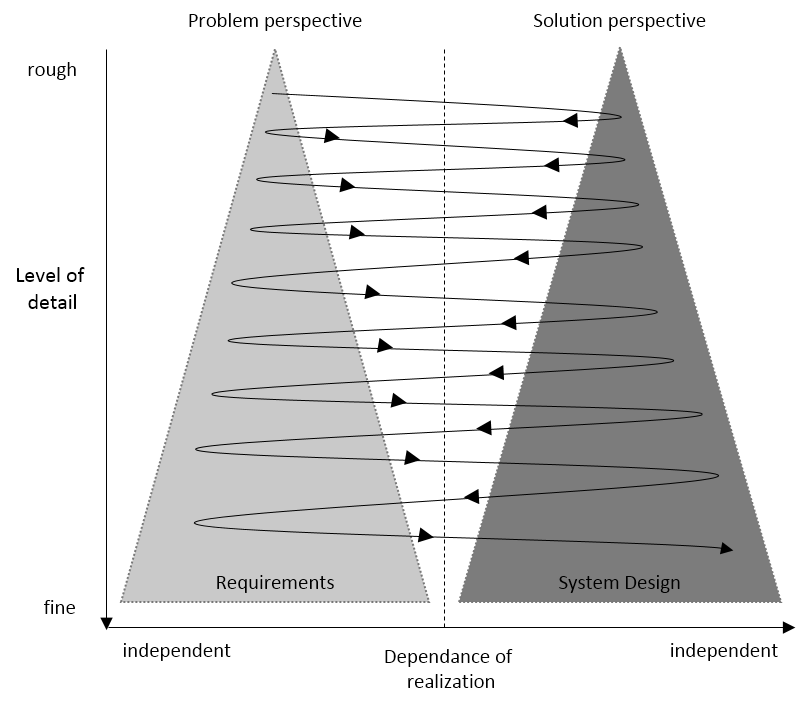
\includegraphics[width=0.7\textwidth]{img/iterative.png}
    \caption[Interdependence of Requirements and Design]{Interdependence of Requirements and Design \parencite[23]{Pohl.2007}}
    \label{fig:iterative}
\end{figure}

\paragraph{} This reflects the iterative nature of requirements engineering as described on \cpageref{iterative}. Thereby each step but the first of the following procedure will end in a check for bidirectional implications of architecture and requirement. The reason for the first step not following a checkup is, that no requirements are formulated yet. 


\paragraph{} This paper will begin with the definition of the context, and then perform the three main activities (cf. \cpageref{mainactivity} and \cpagerefrange{beginmain}{endmain}). In an iterative process, architectural designs will be done, as described above. 


\section{Finding the Context Definition}
This thesis will start the requirement engineering as suggested by \textcite{Pohl.2007} and described in \cref{ssec:reqEn} by gathering information from the requirement sources. For orientation this paper will orientate at the source categories shown in \Cref{fig:reqFlow} on \cpageref{fig:reqFlow} going top down. 

\paragraph{} In the first instance, personas (see below) will be produced, in order to gasp the stakeholders. Withdrawing from the personas and other sources of information - some provided by the sponsor -, goals will be derived into use cases (see below). Those use cases will be analyzed for implications on the facets of the system context, as described on \cpagerefrange{beginFacets}{endFacet}. 


\subsection{Using Personas}
Human brains are caring more bout individuals, than large groups \parencite[cf.][]{Platt.2016}. Therefore, archetypal individual people \parencite[cf.][81-82]{Cooper.2007}, which embody specific characteristics of groups \parencite[cf.][]{Platt.2016} are more easy to gasp. That is the reason for using personas, which do exactly that.

\paragraph{} Identifying, analyzing, and prioritizing personas is a multistage procedure, which is always based on research \parencite[cf.][39]{Robier.2016}. Research methods for this kind do not claim to scientifically accurate, but must not be based solely upon stereotypes and arbitrary decisions \parencite[cf.][82-83]{Cooper.2007}. 

\begin{figure}[H]
\centering
    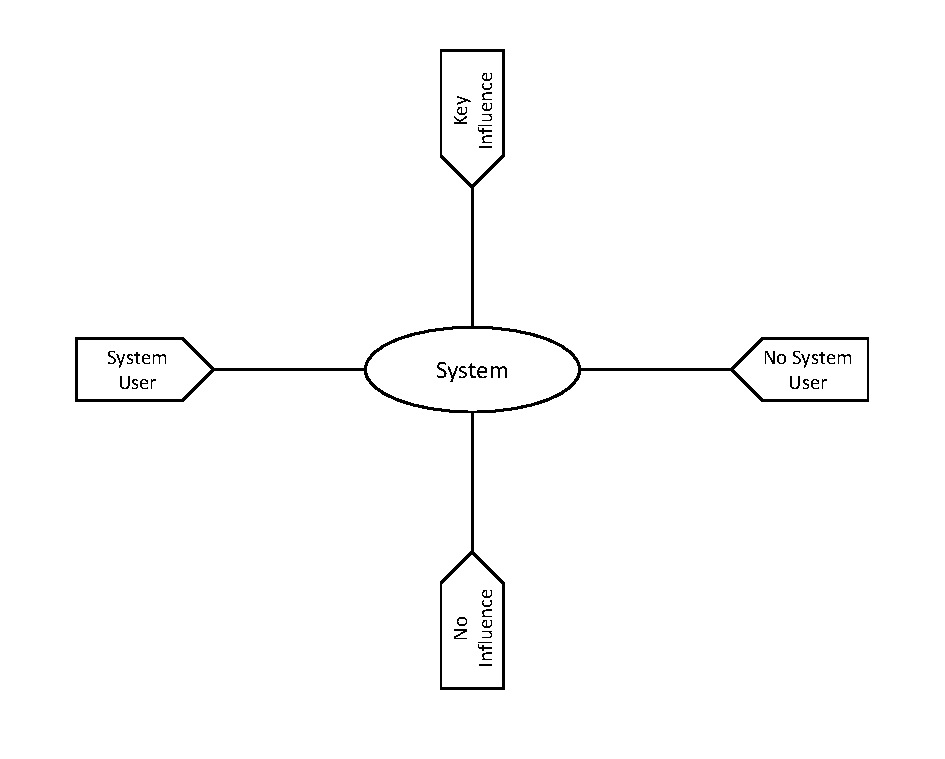
\includegraphics[scale=0.7]{img/stakeholderMap.pdf}
    \caption[Stakeholder Map]{Stakeholder Map (own illustration based on \cite[38]{Robier.2016})}
    \label{fig:stakeMap}
\end{figure}

\paragraph{} For identification of relevant stakeholders \textcite[38]{Robier.2016} suggest the usage of a stakeholder map (cf. \Cref{fig:stakeMap}). People of the left hand side of the vertical axis are the users of the program, divided into heavy users (far left) and fist time users (narrow to the axis) \parencite[cf.][38]{Robier.2016}.
\paragraph{} This approach aims not at the identification of each individual stakeholder, but at the identification of stakeholder groups to be represented by a persona \parencite[cf.][82]{Cooper.2007}, explicitly  including non-users \parencite[cf.][84]{Cooper.2007}.

\paragraph{} Analysis of the personas identified, includes the specification of a personas traits. Since personas are represented as individual people \parencite[cf.][81]{Cooper.2007}, it has all attributes a natural person has, including a name, gender, age, family, education, and most importantly: a motivation \parencites[cf.][]{Platt.2016}[cf.][83-84]{Cooper.2007}. All traits of a persona must be contributing to a bigger picture, and thereby must be intentionally be set to suggest intended characteristics \parencite[cf.]{Platt.2016}. 

\paragraph{} As an example: Our persona Kevin Smith (25, male) works at a international bank as foreign trade manager after his studies in financial management at Harvard Business School and needs a way to plan his meetings in accordance to required travel times. In his free time he has a private single engine plane. If you ask yourself whether Kevin needs his schedule in a standardized time zone, such as UTC, the answer will definitely be yes, because he is on the one hand used to using UTC at work and in his hobby. 

\paragraph{} Martha Jones (55, female) works at a local retailer since her diploma from community college, now being store manager, requiring a tool to plan and distribute shifts of her employees. She on the other hand will have more use for local time. Both may be personas for a calendar service focused on business customers. 

\paragraph{} All traits of Kevin and Martha will have implications on the conception and development of the hypothetical calendar service. Beside the very different functionality requests of transport service provider integration, respectively shift planning and public calendar provisioning, the age may have implications on the devices used, as well as the education implies different kinds of prior knowledge. 

\paragraph{} The prioritization of personas heavily depends on the specific product. It may be done by expected revenue (e.g. for sold services), least specialization (e.g. for training software) or any other reasonable technique for prioritization.

\begin{figure}[H]
    \centering
    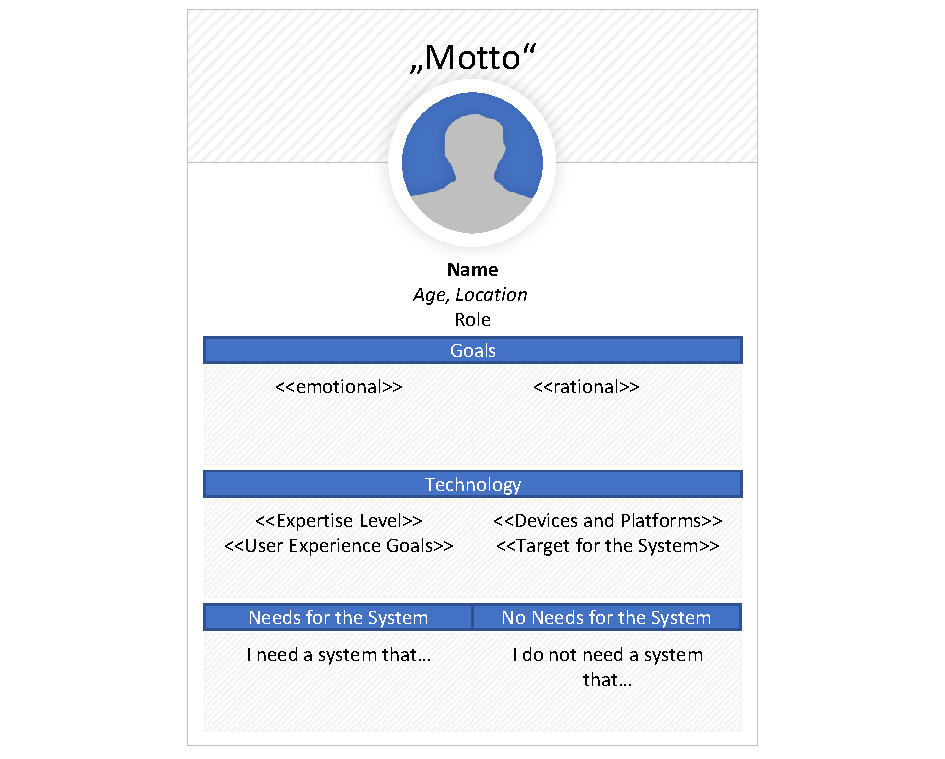
\includegraphics[scale=1]{img/PersonaTemplate.pdf}
    \caption[Template for Personas]{The template used for personas in this paper (own illustration)}
    \label{fig:persTemp}
\end{figure}

\paragraph{} The resulting personas are usually documented in a resume containing all relevant information \parencites[cf.][40]{Robier.2016}[cf.][]{Platt.2016}. This paper will use the template shown in \Cref{fig:persTemp}. It includes a picture of the persona, his or her personal information, his or her goals, needs, and for users his or her technological parameters.


\subsection{Using Use Case Diagrams}
\begin{figure}[H]
    \centering
    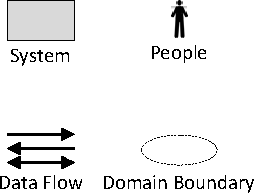
\includegraphics[scale=1]{img/SCDSymbols.pdf}
    \caption[Symbols of System Context Diagrams]{Symbols of System Context Diagrams \parencites[77]{Lauesen.2008}}
    \label{fig:scdSym}
\end{figure}
The system context diagram consists of four components: system, people, data flow, and domain boundaries \parencites[cf.][76-77]{Lauesen.2008}. Each one has its own representation, displayed in \Cref{fig:scdSym}. System context diagrams are used to identify required interfaces \parencites[cf.][75]{Lauesen.2008}, as well as to define the system boundary \parencites[cf.][75]{Ebert.2014}. It is an important overview of requirement sources, reflecting all interacting systems and persons. The direction of the arrow can show the direction of the data flow, or more commonly display the direction of intend \parencite[cf.][77]{Lauesen.2008}. In this paper the direction of an arrow will display the direction of intend.


\section{Main Activity}
\subsection{Sourcing Requirements from the Context}
The information of each facet will be compiled into goals for the desired outcome and which then will be clustered into the types of requirements described in \cref{ssec:reqTypes} (cf. \Cref{fig:reqTypes} on \cpageref{fig:reqTypes}). The formulation of the goals will be done in a sentence stencil (see below) for requirement documentation. 

\paragraph{} The requirements will be itemized and clarified as much as possible to that point. Afterwards, the requirements will be prioritized and potential conflicts will be resolved. The reason for the prioritization before generating consistency is, that in case of an unreasonable conflict, the priorities must be clear to know which requirement to drop.


\subsection{Documenting the Requirements}
\subsubsection{In Natural Language}
Requirements must be expressed distinctly, in order to ensure the system is correctly developed \parencites[107]{Ebert.2014}. While natural language offers great possibilities, being universaly applicable, flexible and easy to use \parencite[cf.][239]{Pohl.2007}, there are some flaws regarding the distinctiveness. Languages have the troubles of containing  ambiguity, which are fatal for distinct communication \parencite[cf.][239-243]{Pohl.2007}.

\paragraph{}
\begin{figure}[H]
    \centering
    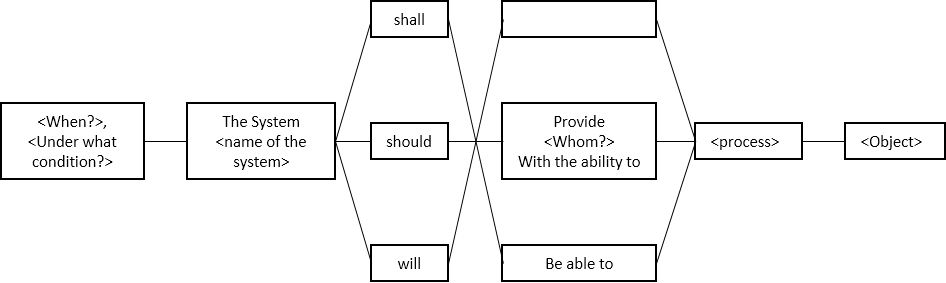
\includegraphics[width=\textwidth]{img/SentenceStructure.png}
    \caption{Requirement Documentation Sentence Structure (own illustration based on \cite[246]{Pohl.2007})}
    \label{fig:sentencestructure}
\end{figure}

In order to counter these issues, this paper will use the sentence structure suggested by \textcites[107]{Ebert.2014}[246]{Pohl.2007}. Sentence structures like these help to clarify and structure requirements, as log as only one requirement is represented per sentence \parencite[107]{Ebert.2014}. 


\subsubsection{In Diagram Notation}
For the diagram documentation of a requirement, a fitting diagram type must be selected \textcite[299]{Pohl.2007}.  This thesis will use use models specified in the Unified Modeling Language (UML) 2.5 documentation by \textcite{ObjectManagementGroup.01.03.2015} with one exception. 

\paragraph{}
Use case diagrams (see below) will be utilized for the documentation of stakeholder's goals. Secondly, this paper will use sequence diagrams, which display the chronological set of interactions, as a tool to visualize scenarios. Last but not least, use cases and scenarios will be merged into function models, which display the flow of information in the complete system and are not part of the UML Specification. 

\begin{figure}[H] 
    \centering
    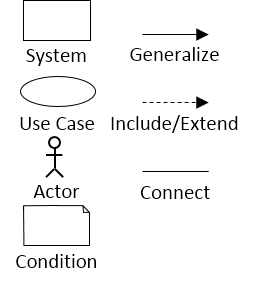
\includegraphics[width=0.28\textwidth]{img/ucSymb.png}
    \subcaption{Use Case Diagram Notation (own illustration based on \cite[163]{Pohl.2007}}\label{fig:ucSymb}
\end{figure}

A use case diagram displays goals of stakeholders by abstracting stakeholders into actors, connected to use cases - abstracted goals -, when interacting with the system. Use case diagrams consist of actors, use cases and the system. It display in what kind the actors are directly or indirectly linked to the use cases. Both, actors and use cases, can be generalized in an aggregated version of themselves. The notation may be seen in \Cref{fig:ucSymb}.

\begin{figure}[H]
    \centering
    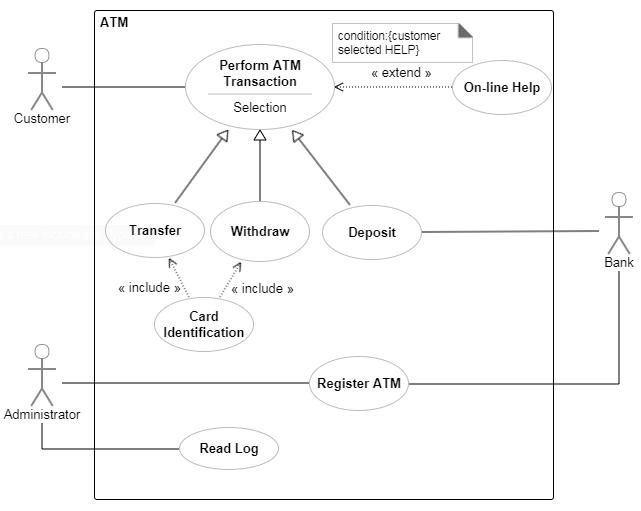
\includegraphics[width=0.73\textwidth]{img/ucEx.png}
    \subcaption[Use Case Diagram Example]{Use Case Diagram Example (own illustrationbased on \cite[641-644]{ObjectManagementGroup.01.03.2015})}\label{fig:ucEx}
\end{figure}

\paragraph{} As an example (cf. \Cref{fig:ucEx}): An Automated Teller Machine (ATM) is used by the \ssay{Customer} with the goal \ssay{Perform ATM Transaction}. This can be either \ssay{Transfer}, \ssay{Withdraw}, or \ssay{Deposit} money. For \ssay{Transfer} and \ssay{Withdraw}, a authentication via \ssay{Card Identification} is included. Including a goal into another means that it must be utilized \parencite[cf.][639]{ObjectManagementGroup.01.03.2015}. 

\paragraph{} If the \ssay{Customer} requires help \ssay{Perform[ing a] ATM Transaction}, the system offers a \ssay{Selection} with the option \ssay{HELP}. This is regarded as a extension of the goal, as the user does not have to make demands on getting helped \parencite[cf.][638-639]{ObjectManagementGroup.01.03.2015}.

\paragraph{} 
Other actors might have completely different goals, when using the ATM, like the Administrator

\paragraph{} As seen in \Cref{fig:ucEx}, the goals do not have to be connected directly to the actor. They might be included in a different goal (e.g. the closet) or may extend other use cases under certain conditions (e.g. ironing equippment).


\begin{figure}[H]
    \centering
    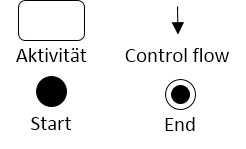
\includegraphics[width=0.7\textwidth]{img/adSymb.png}
    \subcaption{Notation}\label{fig:adSymb}
\end{figure}

\begin{figure}[H] ]{.5\linewidth}
    \centering
    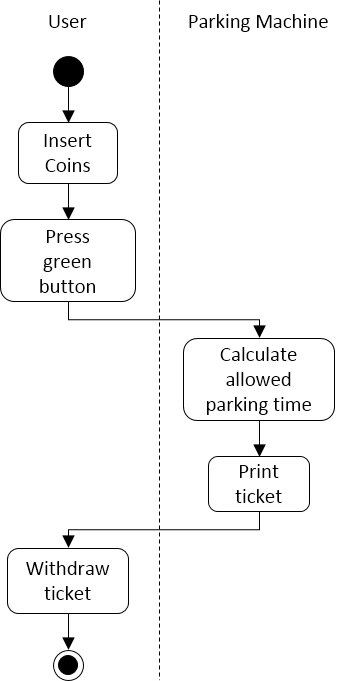
\includegraphics[width=0.9\textwidth]{img/activityDiagram.png}
    \caption{Activity Diagram Example \parencite[380]{ObjectManagementGroup.01.03.2015}}\label{fig:adEx}
\end{figure}

\paragraph{} The activity diagram, on the other hand, expresses a chronological order of activities done by certain entities (system, user, etc.). Those diagrams have one start point and at least to end points, as well as activities, which are connected by control flow lines (cf. \Cref{fig:adSymb}).

\paragraph{} For demonstration \Cref{fig:adEx} shows a activity diagram for a very simple parking ticket machine, as it is commonly used. What this demonstration leaks, is are logical gates such as AND or OR.


\paragraph{} Function models are made to display the 

\paragraph{} 
\begin{figure}[H]
    \centering
    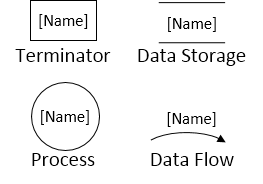
\includegraphics[scale=0.9]{img/fmSymb.png}
    \caption[Function Model Notation]{Function Model Notation (own illustration based on \cite[190]{Pohl.2007})}
    \label{fig:fmSymb}
\end{figure}


\subsection{Validating Conformity}
Scope Out

\section{Architectural Conception}
This paper will use UML component diagrams in the alternate notation \parencite[cf.][212]{ObjectManagementGroup.01.03.2015} for architectural composition of the application. An example of a component diagram can be seen in \Cref{fig:comEx}.

\begin{figure}
    \centering
    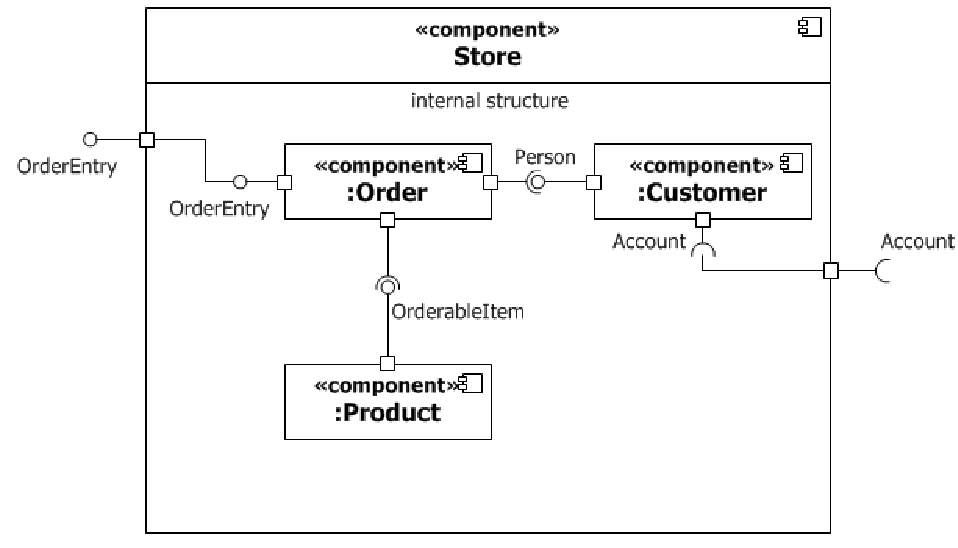
\includegraphics[width=\textwidth]{img/componentExample.pdf}
    \caption[Component Diagram Example]{Component Diagram Example \parencites[2132]{ObjectManagementGroup.01.03.2015}}
    \label{fig:comEx}
\end{figure}

A component in UML notation may be identified either by the keyword \ssay{<<component>>}, or by a component icon in the top right corner \parencites[cf.][208]{ObjectManagementGroup.01.03.2015}. Both is true for \Cref{fig:comEx}. 

\paragraph{} In UML structure diagrams, as the component diagram is, entities follow some basic structures:

\begin{enumerate}
    \item Entities are labeled by a name, and/or are assigned a  classifier by the \ssay{:[classifier]}-notation  \parencite[cf.][125]{ObjectManagementGroup.01.03.2015}. For instance in \Cref{fig:comEx} \ssay{Store} is the name of a component and its inner components are classified as \ssay{Order},\ssay{Customer}, and \ssay{Product}. If \ssay{Store} gets assigned to a classifier (e.g.~\ssay{Business}), the new label will be \ssay{Store :Business}.
    
    \item Components can provide and use interfaces, called ports \parencite[cf.][182-184]{ObjectManagementGroup.01.03.2015}. In \Cref{fig:comEx} the component, classified as \ssay{:Product}, provides the interface \ssay{OrderableItem}, which is used by \ssay{:Order}.
    
    \item Whenever a interfaces is provided to outside components, a square displays the delegation \parencite[cf.][212]{ObjectManagementGroup.01.03.2015}. In \Cref{fig:comEx} for instance, the port \ssay{OrderEntry} is originally provided by some internal logic of \ssay{:Order}, then delegated to \ssay{Store}, which provides it to other external components. 
\end{enumerate}

\section{User Interface Conception}


\subsection{Minimalist Approach of understandable User Interfaces}
Facing the challenges of \textit{Attention Economy}, business decision makers must explore applications at a higher speed that private users, because as stated above, spend attention implies costs of opportunity \parencite[cf.][]{Bakar.2017}. Therefore, designing a application must be done in optimization for fast knowledge transfer and easy exploration. In order to achieve this goal, \textcite{Bakar.2017} suggests a set of goals:
\begin{enumerate}
\item{Getting Started Fast} implies, that no unnecessary contents are disturbing the user from using the core functionality of the page by drastically removing  \say{explanatory and procedural information and let the user learn [...] through exploration} \parencite{Bakar.2017}.
\item{Training on Real Tasks} leads the user more easily receiving information and being more restrained by the application, due to a sense of excitement.
\item{Reading in Any Order} means the quality of the individual information to be not to have perquisite knowledge of any other page within the application.
\item{Exploiting Prior Knowledge} can help to keep the users attention by mostly presenting new information. This is documented as being dificult to be implemented successfully \sekcite{Carroll.1987}{}{Farkas.1990}{}.
\item{Coordinating System and Training} represents the progress of novice users in learning to work with the software. This is accomplished by keeping the users attention on the user interface and supplying constructive information.
\item{Supporting Error Recognition and Recovery} implies strong testing of the application to determine necessary error recognition and implement sufficient information recovery.
\item{Using the Situation} suggest providing the user many ways to explore the application in means of functionality and informational contents. Offering options for preoccupying oneself with the application amplifies the information transfer but increases the potential for errors.
\item{Developing Optimal Training Design} pertains the correlation of the user interface design to the users needs and behaviours. 
\item{Reasoning and Improvising} relatives the approach of explorative interaction by offering instructions where compulsory.
\end{enumerate}


\subsection{Outlining with Wire Frames}


\subsection{Prototyping with Mock-ups}